\section{Reglerentwurf mit Bodediagramm \buchSeite{111}}

\subsection{Phasenreserve und Verstärkungsreserve \buchSeite{112}}
\begin{multicols}{2}
\begin{itemize}
\item Beim Auslegen des offenen Regelkreises sollte neben dem Nominalfall
auch den ‘worst case’ im Auge behalten werden. Auch beim letzteren sollte die
Ortskurve nicht zu knapp neben dem kritischen Punkt vorbei laufen, da dies zu
Resonanzüberhöhungen in den Sensitivitäten S(s) und T(s) führt.
\item Die rechts dargestellten Sicherheitsabstände sind bei den zwei Punkten ablesbar,
wo die Ortskurve den Einheitskreis bzw. die negative reelle Achse durchstösst.
\item Die beiden Punkte entsprechen $G_0(j\omega_D)$ und $G_0(j\omega_{\pi})$, wobei $\omega_D$ die Durchtrittsfrequenz
ist und $\omega_{\pi}$ die Phasenschnittfrequenz.
\item Der erste Punkt liefert die Phasenreserve $\Phi_{RES}$; es gilt $G_0(j\omega_D) = e^{j(-\pi+\Phi_{RES}})$. 
\item Der zweite Punkt liefert die Verstärkungsreserve $K_{RES}$; es gilt $G_0(j\omega_{\pi}) = -1/K_{RES}$. 
\item Der geschlossene Regelkreis wird grenzstabil, wenn im offenen Kreis eine zusätzliche Verstärkung $\widetilde{K} = K_{RES}$ vorhanden ist, d.h. wenn $\widetilde{G}_0 = K_{RES}G_0$.
\item Alternativ wird der geschlossene Regelkreis auch grenzstabil, wenn der offene Regelkreis eine zusätzliche Totzeit $\widetilde{T}_t = \Phi_{RES}/\omega_D$ hat,
d.h. wenn $\widetilde{G}_0 = G_0\cdot e^{-s\cdot\Phi_{RES}/\omega_D}$. Zu beachten ist, dass die beiden Typen von Reserve
miteinander gekoppelt sind.
\end{itemize}
		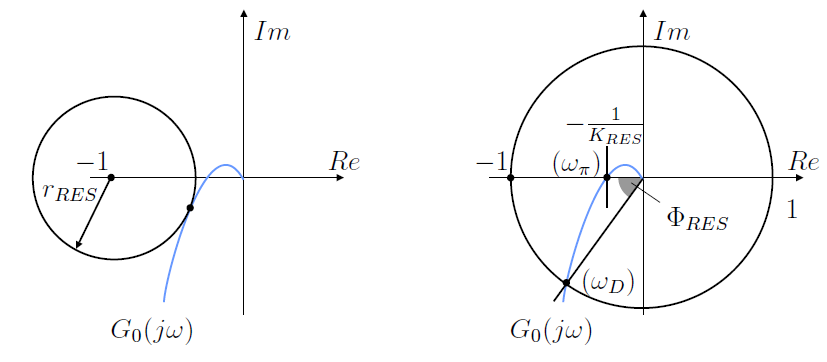
\includegraphics[width=10cm]{./images/PhasenVerstaerkungReserve.png}
\hspace*{2.5cm}Weitere Berechnungen siehe RegT1+2 Buch.
\end{multicols}
\subsection{Spezifikationen für das dynamische Verhalten (II) \buchSeite{115}}
\begin{itemize}
\item Der offene Regelkreis soll das allgemeine Nyquistkriterium
erfüllen, damit der geschlossene Regelkreis stabil wird.
\item Der offene Regelkreis soll ca. eine Phasenreserve $\Phi_{RES}$ zwischen $40^{\degree}$ und $70^{\degree}$
und eine Verstärkungsreserve $K_{RES} > 4 (\approx 12dB)$ aufweisen. Damit wird der
geschlossene Regelkreis robust gegenüber Parameterunsicherheiten und damit
bleiben auch die Überhöhungen von $|S(j\omega)|$ und $|T(j\omega)|$ limitiert.
\item Der offene Regelkreis soll eine hohe Durchtrittsfrequenz $\omega_D$ aufweisen, damit
der Regelkreis eine hohe Bandbreite $\omega_B$ hat und damit ‘schnell’ ist.
\item Die Verstärkung $|G_0(j\omega)|$ des offenen Regelkreises soll bei den tiefen Frequenzen
$\omega < \omega_D$ genug gross sein
\item Im Bereich um die Durchtrittsfrequenz $\omega_D$ sollte $|G_0(j\omega)|$ idealerweise mit
etwa 20 dB/Dekade fallen. Steilere Amplitudengänge in der Umgebung von
$\omega_D$ verkleinern die Phasenreserve $\Phi_{RES}$.\newline
Bei realen Systemen fällt $|G0(j\omega)|$ für $\omega \geqslant \omega_D$ mit mindestens 40 dB/Dekade
ab, weil sowohl Strecke wie Regler Tiefpassverhalten haben.
\end{itemize}
\subsection{Entwurfsbeispiele \buchSeite{116}}
\paragraph{Inverse Regler \buchSeite{116}} \mbox{} \\

    Dass der Regler die Inverse der Strecke enthält, ist ein gängiges Konzept. Allerdings
    kann es oft nicht vollständig umgesetzt werden. Beispielsweise darf die Strecke weder
    Pole noch Nullstellen in der rechten Halbebene haben und auch keine Totzeit enthalten

\paragraph{$\mathbf{PIDT_1}$ \buchSeite{116}}

\paragraph{Lead/Lag-Glied \buchSeite{118}}

    \begin{minipage}{6cm}
        \[ G(s) = K \cdot \dfrac{sT_1+1}{sT_2+1} \]
    \end{minipage}
    \begin{minipage}{8cm}
        Lead-Glied: $T_1 > T_2 > 0$ \newline
        Lag-Glied: $T_2 > T_1 > 0$ 
    \end{minipage}

\paragraph{Notch-Filter \buchSeite{120}}

%Schritte des Reglerentwurfs kann man sich so vorstellen
%\begin{itemize}
%\item  Der Reglerpol bei Null erzeugt bei $G_0$ die gewünschte grosse Verstärkung bei
%tiefen Frequenzen.
%\item  Die beiden Nullstellen des Regler ‘biegen’ die Kurve von $|G_0(j\omega)|$ gerade, so
%dass sie durchgehend mit 20 dB/Dekade fällt. $G_0(j\omega)$ ist jetzt konstant $-90^{\degree}$.
%Der offene Regelkreis entspräche der Idealsituation eines Integrators.
%\item  Wegen der Realisierbarkeit muss noch ein zweiter Reglerpol eingeführt werden,
%der $|G_0(j\omega)|$ bei der - relativ hohen - Frequenz $\omega$ = 20 [rad/s] wieder nach
%unten knickt und der die Phase $G_0(j\omega)$ bei höheren Frequenzen auf $-180^{\degree}$
%fallen lässt.
%\item  Mit der Verstärkung KR wird die Phasenreserve $\Phi_{RES} = 65^{\degree}$ eingestellt.
%\end{itemize}


\subsection{Bemerkungen zum Reglerentwurf mithilfe von Spezifikationen \buchSeite{122}}

Zu beachten ist, dass es einige fundamentale Einschränkungen für die Bandbreite
von Regelkreisen gibt. Folgende Abschätzungen zu
instabilen und nichtminimalphasigen Systemen:
\begin{enumerate}
\item Eine Strecke hat einen \textbf{reellen Pol p in der rechten Halbebene}. 

Will man in diesem Fall $T(j\omega) \leq 2$ halten (6 dB), muss die Bandbreite $\omega_B$
einen Mindestwert haben:
\[\omega_B > 2p\]
\item Eine Strecke hat eine \textbf{reelle Nullstelle z in der rechten 
Halbebene}.

Will man in diesem Fall eine Phasenreserve von ca. $35^{\degree}$ erreichen, muss die
Durchtrittsfrequenz $\omega_D$ limitiert werden (und damit auch die Bandbreite $\omega_B)$ \[\omega_D < z/2\]

\item Eine Strecke hat eine \textbf{Totzeit} $T_t$

Um in diesem Fall eine Phasenreserve von ca. $35^{\degree}$ zu erreichen, muss die Durchtrittsfrequenz
$\omega_D$ limitiert werden (und damit auch die Bandbreite $\omega_B$):
\[\omega_D < 1/T_t\]
\end{enumerate}
Offensichtlich gibt es also auch Situationen, in denen das Lockern von Spezifikationen
gar nichts hilft; etwa bei Kombination von Fall 1 mit Fall 2. Um einen sinnvollen
Regler entwerfen zu können, muss primär die Regelstrecke modifiziert werden.
